\documentclass[10pt]{article}
\usepackage[a4paper,margin=1.6cm,top=1.3cm,bottom=1.3cm]{geometry}
\usepackage[T1]{fontenc}
\usepackage{lmodern}
\usepackage{microtype}
\usepackage{booktabs}
\usepackage{graphicx}
\usepackage{enumitem}
\usepackage{xcolor}
\usepackage[colorlinks=true,linkcolor=black,citecolor=black,urlcolor=blue]{hyperref}
\setlist{nosep,leftmargin=1.2em,topsep=1pt}
\setlength{\parindent}{0pt}
\setlength{\parskip}{3pt}
\pagestyle{empty}
\newcommand{\head}[1]{\par\smallskip{\large\bfseries #1}\par}
\newcommand{\sect}[1]{\par\smallskip{\bfseries\color{black!80} #1}\par}

\begin{document}
\head{Idea 6 PoC --- Sticky analyst expectations and the profitability anomaly}
\textit{Proof of concept, October 2026. Code: \texttt{idea06\_sticky\_expectations/run.py}.}

\sect{Question and design}
Bouchaud, Krueger, Landier and Thesmar (2019, JF) explain the US profitability anomaly with sticky expectations:
forecasters update too slowly, stay too pessimistic about profitable firms, and the premium is larger where
expectations are stickier. Does this hold in China? The sample is I/B/E/S-covered firm-months, 2005--2020. The
consensus error is $FE_m=(R_m-F_m)$, where $F_m$ is the price-scaled 12-month-forward consensus and $R_m$ the
I/B/E/S trailing EPS twelve months later. ROE is \emph{realised} TTM EPS divided by book value per share. The
bonus-adjusted EPS is first converted back to each month's share basis, using share events inferred from the price
and total-return series. Firm-level stickiness is proxied by the autocorrelation of the firm's monthly consensus
revisions over the previous 24 months; sticky updating spreads news over several revisions. All return tests are
next-month, with Newey--West $t$-statistics.

\begin{center}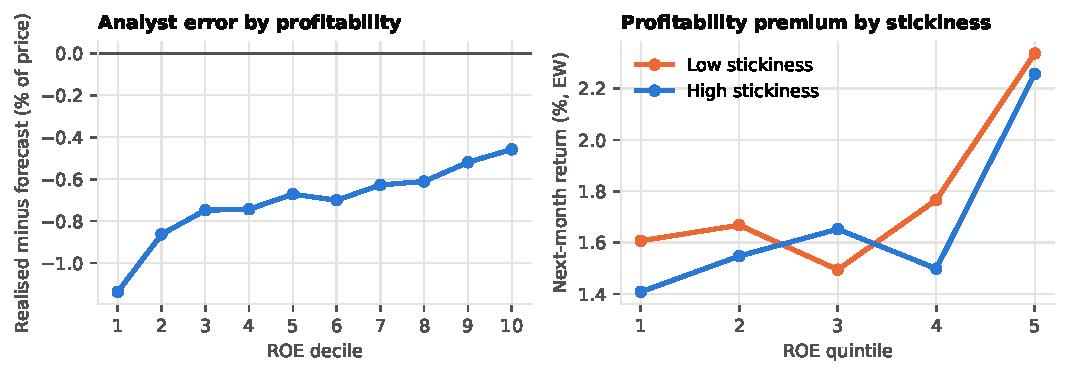
\includegraphics[width=0.97\textwidth]{results/fig_main.pdf}\end{center}

\begin{center}\small
\begin{tabular}{llc}
\toprule
Test & Specification & Estimate ($t$)\\
\midrule
Consensus underreaction (CG) & $FE$ on 3-month revision, all & 0.14 (2.5)\\
 & \quad high-stickiness firms / low-stickiness firms & 0.28 (4.3) / 0.04 (0.6)\\
Pessimism about profitable firms & $FE$ on ROE & 0.006 (2.0)\\
Profitability anomaly & ROE quintiles, Q5$-$Q1 raw / CH-4 $\alpha$ (\%/month) & 0.90 (3.3) / 0.57 (2.0)\\
 & FM slope per 1 SD of ROE, with controls & 0.21 (2.9)\\
Role of stickiness & Q5$-$Q1, high minus low stickiness & 0.12 (0.4)\\
 & FM interaction ROE $\times$ stickiness & 0.01 (0.1)\\
Forecast-contaminated ROE & I/B/E/S trailing EPS / BV, FM slope & $-0.36$ ($-5.0$)\\
 & jointly: realised ROE / I/B/E/S ROE & 0.60 (8.6) / $-0.62$ ($-8.0$)\\
\bottomrule
\end{tabular}
\end{center}

\sect{Findings}
\begin{itemize}
\item \textbf{The consensus is sticky, and the proxy finds where.} Forecast errors follow the direction of recent
  revisions (CG slope 0.14), confirming Li and Li (2025) on our data. The slope is concentrated in firms whose past
  revisions are autocorrelated (0.28 against 0.04), which validates the stickiness proxy out of sample.
\item \textbf{The profitability anomaly exists in China,} at about 0.6--0.9\% per month, and analysts are
  \emph{relatively} too pessimistic about profitable firms, as in the US. However, Chinese analysts are optimistic
  everywhere: by 1.1\% of price for the lowest ROE decile and 0.5\% for the highest.
\item \textbf{Stickiness does not explain the anomaly here.} The premium is the same for sticky and non-sticky
  firms, so the cross-sectional prediction of Bouchaud et al.\ fails with this proxy.
\item \textbf{The measurement trap is itself a finding.} ``ROE'' built from the I/B/E/S trailing field, which blends
  in forecasts, predicts returns with the \emph{opposite} sign. Controlling for realised ROE, the forecast part
  predicts low returns, the same optimism effect as in Idea 5.
\end{itemize}

\sect{Assessment and next steps}
Publishable only with a better stickiness measure. Bouchaud et al.\ estimate it at the analyst level, which needs
I/B/E/S detail data (individual forecasts and revisions). The most promising angle is the asymmetry: optimism
concentrated in unprofitable firms, and whether it explains the low returns of low-ROE stocks. This overlaps with
Idea 5, so the two could merge into one paper on analyst optimism and anomalies in China.
\end{document}
